\documentclass[a4paper, 15pt, openright, twoside]{article}

\usepackage{graphicx}
\usepackage{polski}
\usepackage[english,polish]{babel}
\usepackage[utf8]{inputenc}
\usepackage[top=3.5cm,bottom=4.5cm,left=3.5cm,right=3.5cm, bindingoffset=0cm, footskip=2.5cm]{geometry}
\usepackage{setspace}
\usepackage{multirow}
\usepackage{mwe}
\usepackage{blindtext}
\usepackage{caption}
\usepackage{float}
\usepackage{chngcntr}
\addto\captionsenglish{% Replace "english" with the language you use
	\renewcommand{\contentsname}%
	{Table of contents}%
}
\usepackage{dblfloatfix}
\usepackage{lipsum}

%\selectlanguage{polish}
\usepackage{tocloft}
\renewcommand{\cftsecleader}{\cftdotfill{\cftdotsep}}
\renewcommand{\cftdot}{.}
\renewcommand*{\numberline}[1]{}
\usepackage{etoolbox}
\usepackage{titlesec}

\begin{document}

\counterwithin{figure}{subsection}
\selectlanguage{english}
\begin{titlepage}

\begin{center}

%
\includegraphics[scale=1.25]{agh_nzw_s_pl_1w_wbr_pms}\\[0.2cm]

\includegraphics[scale=1.25]{agh_nzw_s_en_1w_wbr_pms}\\[0.2cm]

\textbf{\scriptsize  FACULTY OF COMPUTER SCIENCE,  ELECTRONICS AND TELECOMMUNICATIONS}\\[0.2cm]

\textsc{\scriptsize DEPARTMENT OF TELECOMMUNICATIONS}\\[1cm]

\textbf{\small Engineering Thesis}\\[1cm]

{\huge Impact of Periodic Interference on IEEE 802.11ax Networks}\\[0.5cm]
{\huge Wpływ cyklicznych interferencji na działanie sieci standardu IEEE 802.11ax}\\

\vfill

\begin{minipage}{0.8\textwidth}
\begin{flushleft}
{\large \emph{AUthor:} \hfill Filip \textsc{Nożkiewicz}}\\[0.1cm]
{\large \emph{Degree programme:} \hfill \textsc{ICT}}\\[0.1cm]
{\large \emph{Supervisor:} \hfill Szymon Szott PhD\textsc{}}
\end{flushleft}
\end{minipage}\\[2cm]

Kraków 2019

\end{center}

\end{titlepage}


\textit{
Uprzedzony o odpowiedzialnosci karnej na podstawie art. 115 ust. 1 i 2 
ustawy z dnia 4 lutego 1994 r. o prawie autorskim i prawach pokrewnych
(t.j. Dz.U. z 2006 r. Nr 90, poz. 631 z późn. zm.): „Kto przywłaszcza sobie autorstwo albo wprowadza w błąd co do autorstwa całosci lub częsci cudzego utworu albo artystycznego wykonania, podlega grzywnie, karze ograniczenia 
wolności albo pozbawienia wolności do lat 3. tej samej karze podlega, kto rozpowszechnia bez podania nazwiska lub pseudonimu twórcy cudzy utwór w wersji oryginalnej albo w postaci opracowania, artystycznego wykonania albo publicznie zniekształca taki utwór, artystycznego wykonanie, fonogram, wideogram lub nadanie.", a także uprzedzony o odpowiedzialności dyscyplinarnej na podstawie art. 211 ust. 1 ustawy z dnia 27 lipca 2005 r. Prawo o szkolnictie wyższym (t,j, Dz. U. z 2012r. poz. 572, z późń. zm.):
"Za naruszenie przepisów obowiązujących w uczelni oraz za czyny uchybiające godności studenta student ponosi odpowiedzialnośc dyscyplinarną przed komisją dyscyplinarną albo przed sądem koleżeńskimsamorządu studenckiego, zwanym dalej <<sądem koleżeńskim>>.",oświadczam, że niniejszą pracę dyplomową wykonałem(-am) osobiście i samodzielnie i że nie korzystałem(-am) ze źródeł innych niż wyienione w pracy.
}

\thispagestyle{empty}
\vspace{10in}


\thispagestyle{empty}
\
\vfill

\begin{flushright}

\begin{minipage}{0.65\textwidth}

\textit{I would like to express my sincere gratitude to my
supervisor, Szymon Szott, for the continuous support and guidance during research and writing of this thesis.}\\

\raggedleft \ \\[0.2cm]
\
\end{minipage}

\end{flushright}



\newpage\phantom{}
\tableofcontents
\newpage\phantom{}
\section{1. Introduction}
\section{2. Background}
\section{3. Testbed description}
\textnormal{
	\hspace*{0.5cm}Doing Researches require proper testing environment, which is able to run required test-cases and is relatively comfortable to use.
	The vital thing is that the results must be reliable and can give desired conclusions about particular problems. In this case ns-3 simulator has been chosen. This chapter focuses on an overview of this tool and scenario prepared using it.}
\subsection{\hspace*{0.5cm}3.1 Overview of the ns-3 simulator}
\textnormal{\hspace*{0.5cm}Ns-3 simulator is an open source tool written in C++ programming language with bindings available for Python.It is targeted primarily for research and educational use and is under license of GNU GPLv2. Ns-3 is a discrete-event simulator, so models the operation of a system as a discrete sequence of events in time. Interface of this tool are files with extension of 'cc' or 'py', so models and simulations are directly written in C++ or Python programming languages. Simulation's events are executed in order which is determined by scheduler and the simulation stops when all of the events finish. There is a documentation for ns-3 available on it's official page as well as many scripts and examples. The only operating system which is supported by ns-3 is a Linux. During writing of the thesis 'Ubuntu 16.0.54 LTS' version was used and the version of simulator was 3.29.}
\subsection{\hspace*{0.5cm}3.2 Scenario description}

\textnormal{\hspace*{0.5cm}In order to research specified in the title of the thesis, the particular scenario has been configured. The conditions of simulation's were dynamically changing so automation was needed to run simulation relatively fast and without additional manual chcnages in test scenario. There were separated tools involved to observe specific behaviours and analyze results like statistics libraries of python and wireshark. Everything had to be done in a proper order starting from configuring the scenario, writing automation script and proceeding and analyze essential data produced in time of simulation.}
\subsubsection{\hspace*{0.5cm}3.2.1 Topology}
	\textnormal{\hspace*{0.5cm}Topology consists of two wireless Access Points. The first one is to receive traffic from slow stations and the second one from fast stations. Slower stations send data with much lower rate. Simulation scenario includes those 2 types of stations to observe different explore how stations with completely different data rates behave when it comes to share frequency range with LTE signals. There are also cases where there is  only one Access Point. The number of stations is variable and can be changed whenever it is needed also while simulation is running. Each staion send data to it's own access point.\newline\hspace*{1cm}Essential part of the topology is an interferer which is configured to act as a LTE base station and generate signals which interfere with 802.11 transmission. In some scenarios Interferer must be excluded so and then it's transmit power is decreased to zero. Basic Topology is shown in Figure 3.1. }
	\begin{figure}[h]

	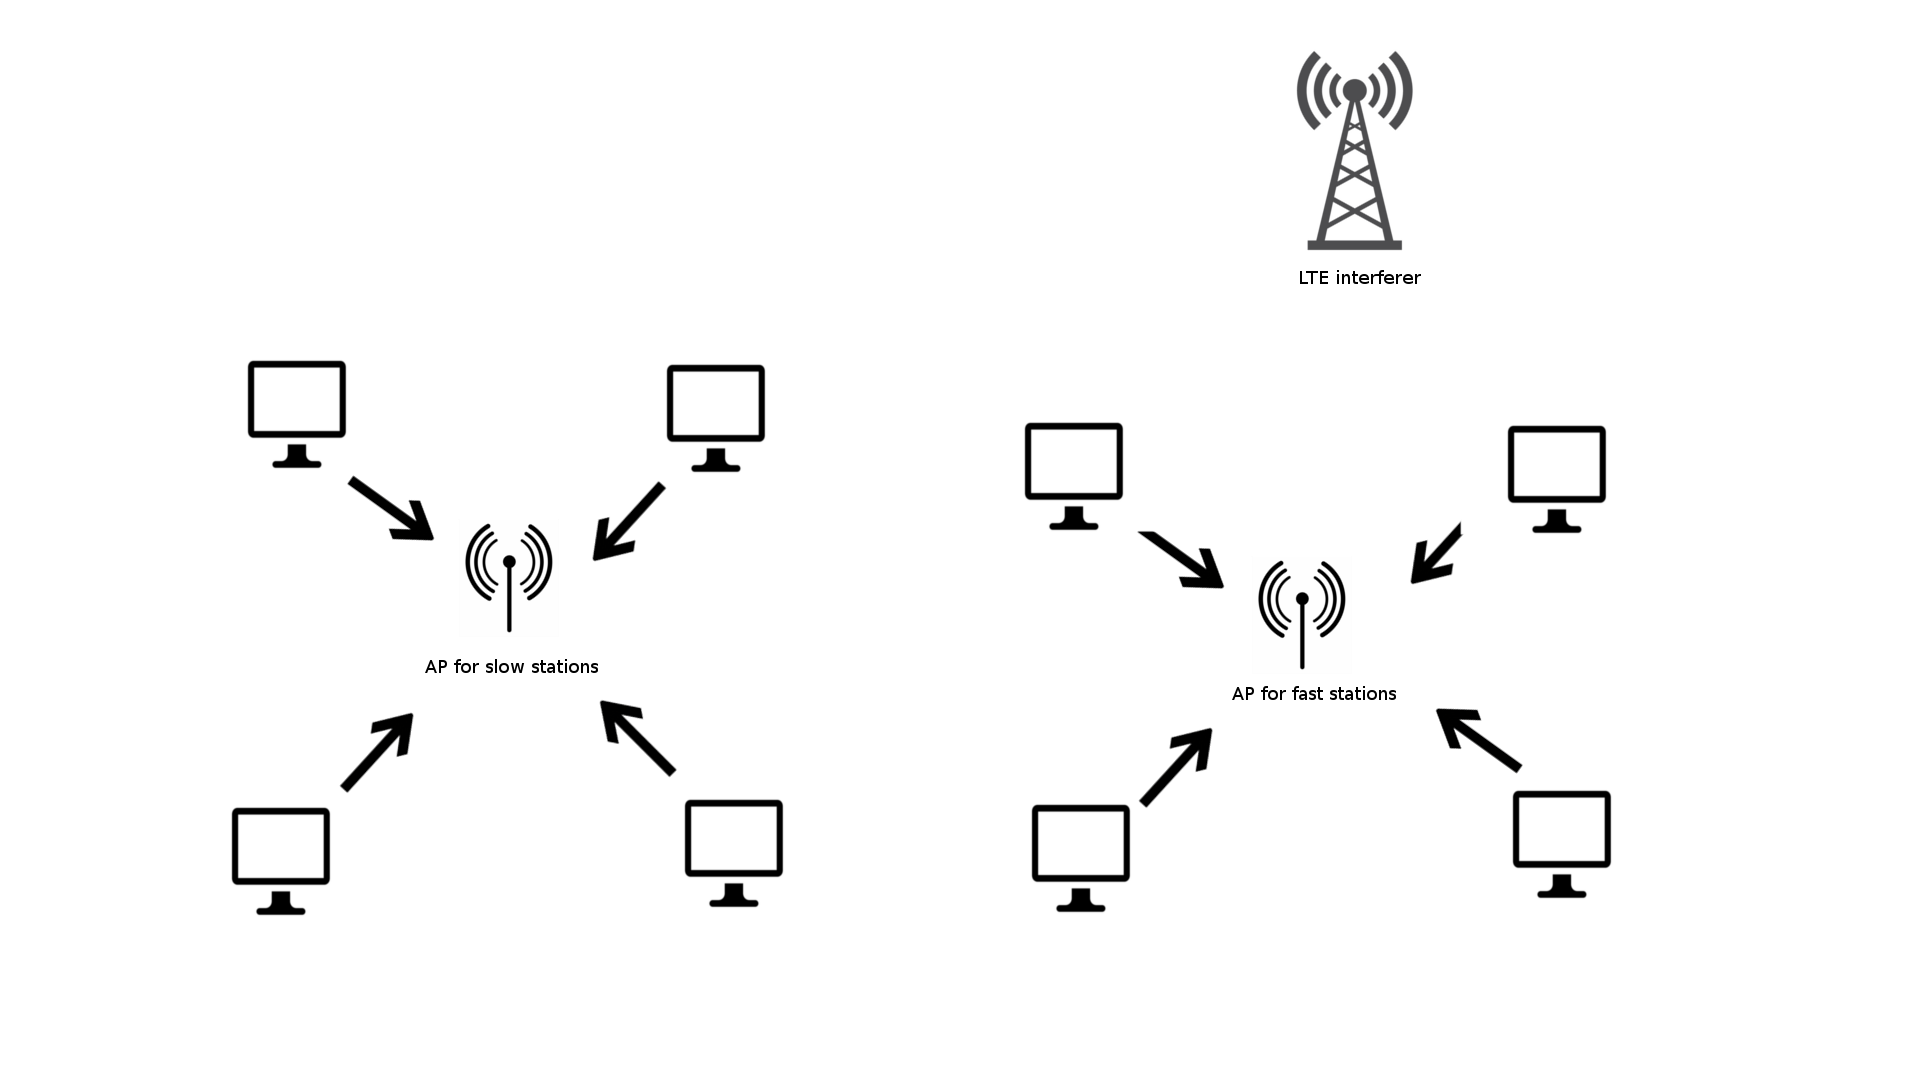
\includegraphics[scale=0.25]{Images/topology}
	\caption{Basic topology}
	\end{figure}
	
\subsubsection{\hspace*{0.5cm}3.2.2 Code description}
\textnormal{\hspace*{0.5cm}Figure 3.2 shows part of the code which is responsible for generating particular frequency range which is used during simulation and specific channel width. In 802.11 ax channel width can be choosen from 20 MHz, 40 MHz, 80 MHz, 80+80 MHz and 160 MHz. }

\begin{center}
	\begin{figure}[!h]	
		\centering
		\fbox{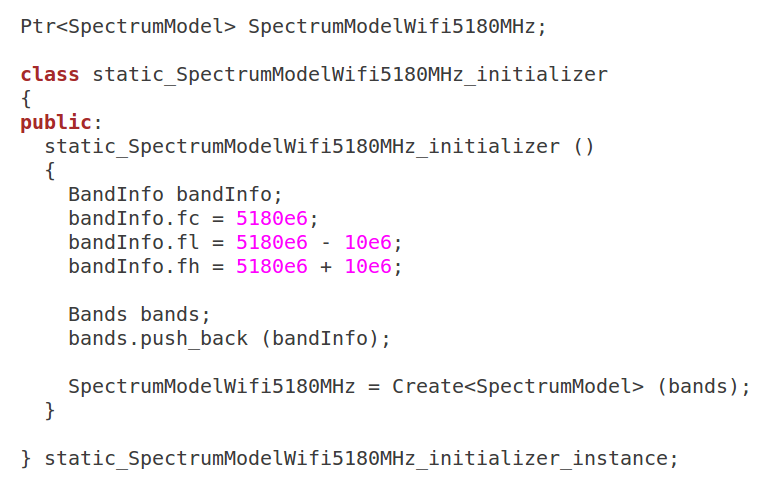
\includegraphics[scale=0.38]{Images/frequencyset}}
		\caption{Spectrum generator}
	\end{figure}
\end{center}
\newpage\phantom{}	
\textnormal{\hspace{0.5cm}Next essential step was to configure Physical layer. Figure 3.2.3 demonstrate sample settings with built-in class WifiHelper. On this stage must be set parameters like MCS (modulation coding scheme), fragmentation treshold and any other parameter which is strictly connected to physical layer. PrpagationLossModel and PropagationDelayModel are  classes provided by ns-3 which models the propagation loss and delay thrue the transmission medium. }
	\begin{center}
		\begin{figure}[h]
		\centering
		\fbox{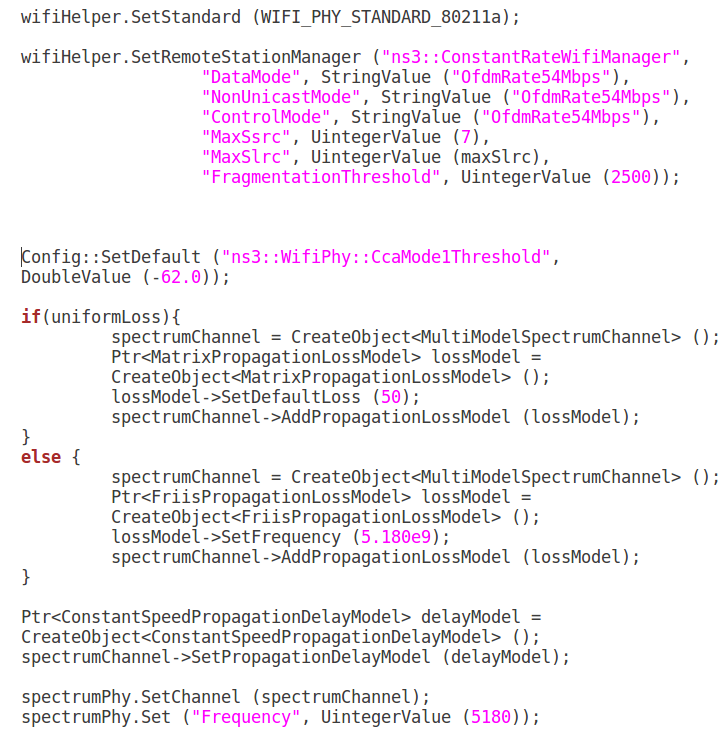
\includegraphics[scale=0.50]{Images/propagationmodel}}\\
		\caption{physical layer settings}
		\end{figure}
	\end{center}  
\textnormal{\hspace{0.5cm}Network layer configuration consisted of creating separated ipv4 address range for slow stations and fast stations and setup arp caching in order to make communication between data link layer and network layer possible . Configuration of network layer illustrates Figure 3.2.4.}
\begin{center}
	\begin{figure}[h]
	\centering
	\fbox{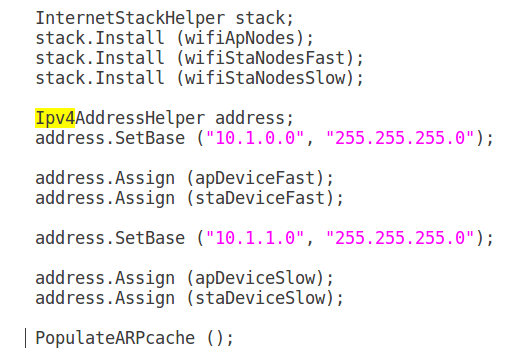
\includegraphics[scale=0.50]{Images/networklayer}}\\
	\caption{network layer configuration}
	\end{figure}
\end{center}  
\textnormal{\hspace{0.5cm}Transport and Application layer were configure in a single function. Ns-3 has built-in class called InetSocketAdress which was used to create layer 4 socket using port and address of specific node. This 2 values were being incremented and assign to each station. All the data transmission was done with UDP protocol. Application layer has been configured with ApplicationContainer class which allow to set required time to start and optional time to stop simulation.\newline\newline}

 \textnormal{\hspace{0.5cm}Lte interferer was created due to the WaveformGeneratorHelper class. It is used to inject specific noise to the channel. It allows to set Spectral power density and physical parameters like period and dutycycle. Finally is installed on a NetDeviceContainer which includes all configured stations. After that when specific lever of power is set waveformgenerato is able to disrupt wifi transmission. Sample settings are presented in Figure 3.2.5.} 
 \begin{center}
 	\begin{figure}[h]
 		\centering
 		\fbox{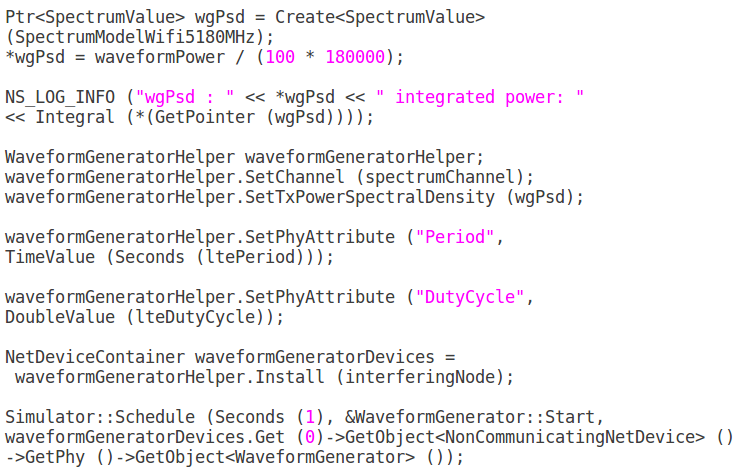
\includegraphics[scale=0.38]{Images/lte}}\\
 		\caption{LTE interferer configuration}
 	\end{figure}
 \end{center}  
\subsubsection{\hspace*{0.5cm}3.2.3 Input parameters}
\textnormal{\hspace{0.5cm}To make simulations more comfortable to use and overall process more efficient group of parameters had been defined. Those parameters were being changed before and while running simulation due to the automation process. Their values needed to be present in output results in order to group data by specific values. Parameters are presented in Figure 3.2.7.}
\begin{center}
	\begin{figure}[h]
		\centering
		\fbox{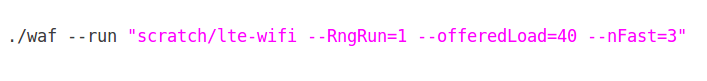
\includegraphics[scale=0.38]{Images/param}}\\
		\caption{Run simulation script with command line arguments}
	\end{figure}
\end{center}
\begin{center}
	\begin{figure}[h]
		\centering
		\fbox{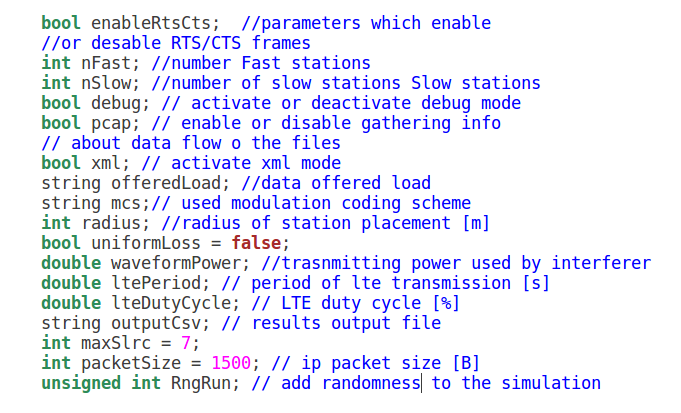
\includegraphics[scale=0.38]{Images/param_table}}\\
		\caption{Configuration parameters}
	\end{figure}
\end{center}    
\subsubsection{\hspace*{0.5cm}3.2.4 Flow Monitor}
\textnormal{\hspace{0.5cm}FlowMonitorHelper is a class in ns-3 which helps to enable ip monitoring on a set of nodes. Iw was used in all of the simulation. FlowMonitor has 'starttime' attribute which is usually set to value larger than 'starttime' of simulation because there is a need to wait a warmup time to get only reliable data. Data were being  dumpded to the csv files during simulation run. Ipv4FlowClassifier is a tool which helped to properly classify data before dumping it to the file. This class differentiate single flows by their parameters. Packets are assigned to specific flows and Flow is characterized by Five element tuple (Source IP , Destination IP , Source Port , Destination Port , Transport Layer Protocol) . Classifier check what is the time of first and last transmitted packet as well as first and last received packet , check numjber of packets being transmitted and received which is usefull to count loss. Parameters which were given as an input are also taken into account because they are assigned to particular flows. Figure 3.2.8 presents configuration of the classifier and Figure 3.2.9 part of the csv file with gathered simulation data. }
\begin{center}
	\begin{figure}[h]
		\centering
		\fbox{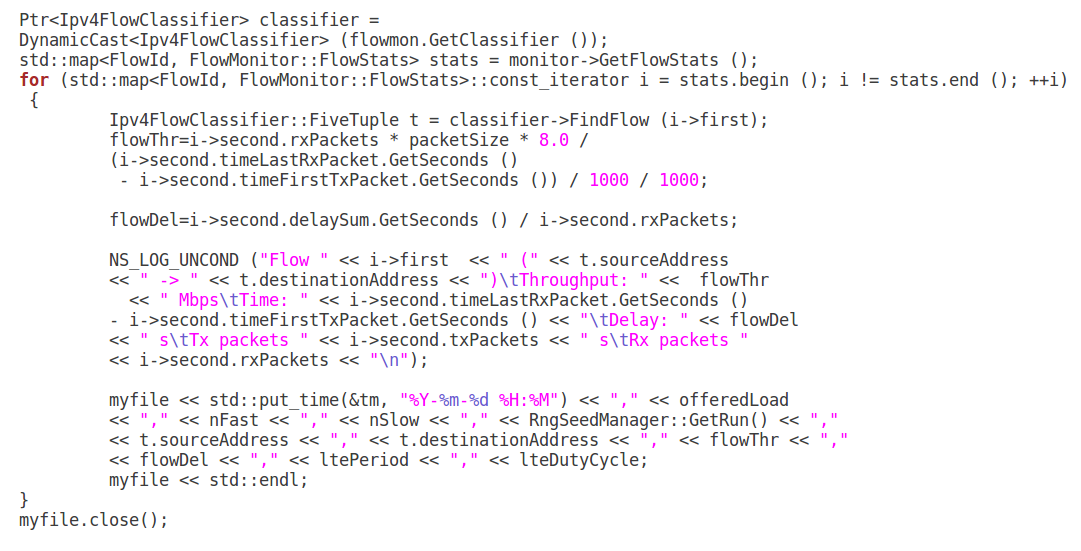
\includegraphics[scale=0.40]{Images/classifier}}\\
		\caption{Run simulation script with command line arguments}
	\end{figure}
\end{center}
\begin{center}
	\begin{figure}[h]
		\centering
		\fbox{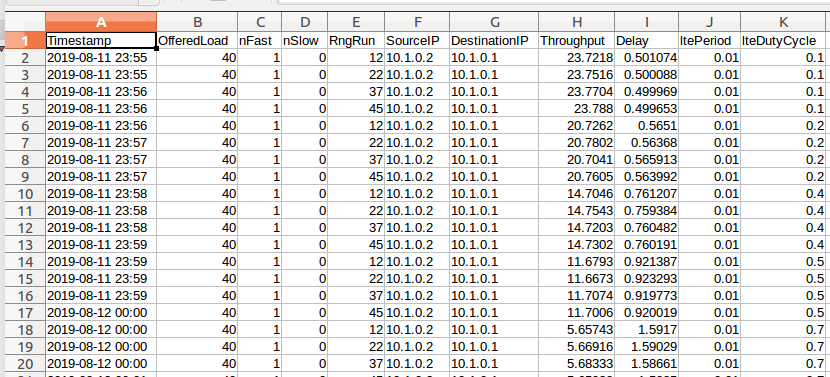
\includegraphics[scale=0.47]{Images/data}}\\
		\caption{Configuration parameters}
	\end{figure}
\end{center}    
\newpage\phantom{}
\subsubsection{\hspace*{0.5cm}3.2.5 Automation}
\textnormal{\hspace{0.5cm}To run simulations without constant manual changes, automation scripts were created. Because ns-3 works on a Linux operating system scripts were written in bash. The process of automation consist of defining sets of parameters and loops inside which were commands starting simulation scenario with parameters from previously define sets. Results were usually appended to the csv file and when simulation were finished data were proceeded and analyzed with python script. Python scripts were based mostly on modules like pandas, matplotlib and scipy. Scripts generated plots and graphs which presented data in a form that enable to find dependencies between them and draw final conclusions. }
\begin{center}
	\begin{figure}[h]
		\centering
		\fbox{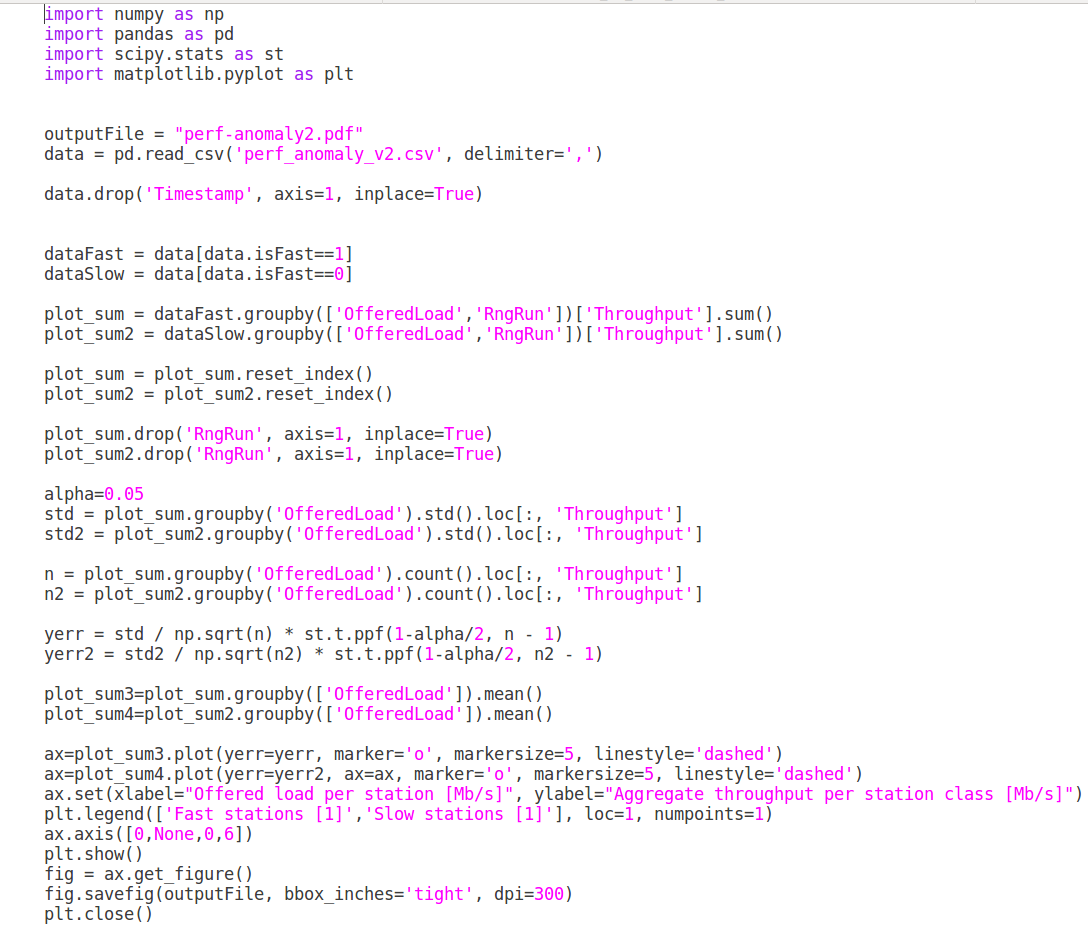
\includegraphics[scale=0.28]{Images/python}}\\
		\caption{Sample python script for data analysis}
	\end{figure}
\end{center} 
\begin{center}
	\begin{figure}[h]
		\centering
		\fbox{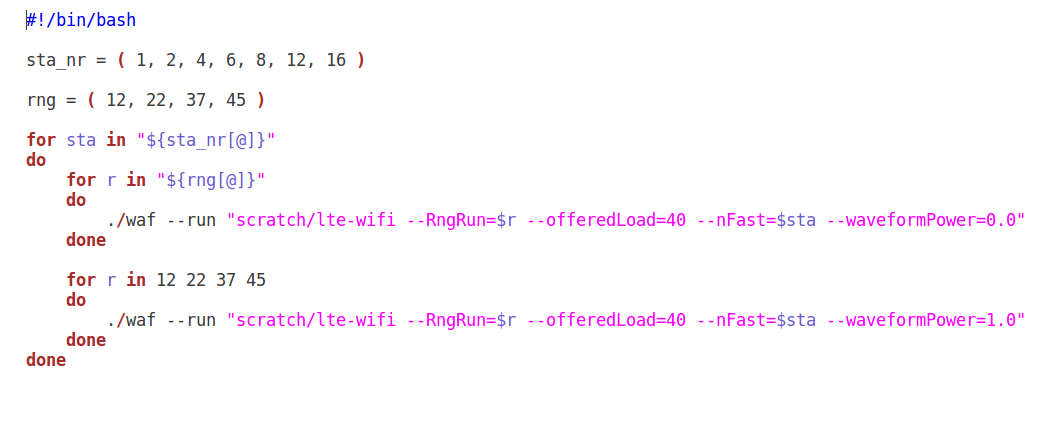
\includegraphics[scale=0.30]{Images/bash}}\\
		\caption{Sample automation script in bash}
	\end{figure}
\end{center}

\newpage\phantom{}

\section{4. Simulations and Analysis}
\section{5. Summary and Conclusions}

\appendix
\end{document}
